% Chapter 1

\chapter{Organisation de l'équipe et planning} % Main chapter title

\label{Chapter1} % For referencing the chapter elsewhere, use \ref{Chapter1}

%----------------------------------------------------------------------------------------

\section{Organisation de l'équipe}

Afin de se concentrer sur la "Solution n°2" lundi 8 nous nous sommes tous lancés dans
l'annalyse du code c du driver et du déroulé de son fonctionnement. Le code réparti
entre chacun, nous avons cherché à comprendre les utilité des structures et de
l'organisation d'un client kernel. Nous avons donc chacuns poursuivit les appels
aux fichiers systemes, en mutualisant les informations oralement.

Grâce à cette agile organisation nous avons pu préciser la source du problème
avant d'en chercher la solution.

Par la suite Romain suivi par Alan se sont lancés dans le second objectif
d'évolution, la compilation d'un noyau en version 4.14. Ce afin de précéder le
portage du driver à ce kernel.

\section{Planning}

Ci-dessous, un planning des tâches effectuées en 2018.

\begin{figure}[th]
    \centering
    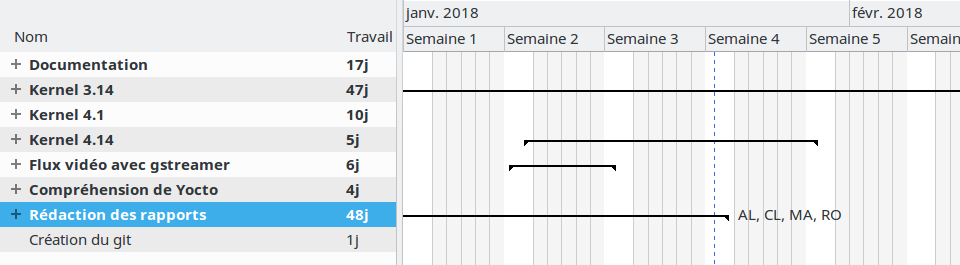
\includegraphics[width=1\linewidth]{planning_petit.png}
    \decoRule
    \caption{Avancement général du projet}
    \label{fig:planning}
\end{figure}
\begin{figure}[th]
    \centering
    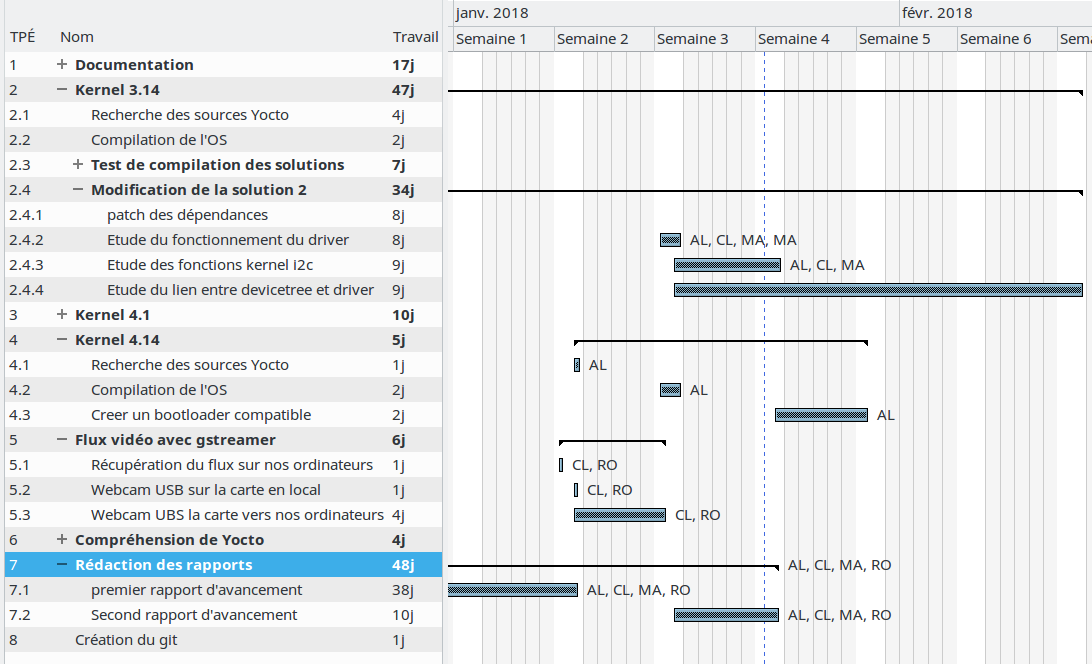
\includegraphics[width=1\linewidth]{planning_grand.png}
    \decoRule
    \caption{Avancement détaillé du projet}
    \label{fig:planning}
\end{figure}

\begin{description}
  \item[AL =] Alan Ait-Ali
  \item[MA =] Martin LAPORTE
  \item[RO =]  Romain Petit
  \item[CL =] Clément Ailloud
\end{description}

La totalité du planning est accessible sur notre git, sur la branche "presentation"
à l'emplacement "meta-openrexpicam/presentation2/gantthales.planner" sous forme
de fichier à ouvrir avec le logiciel "planner" (sudo aptitude install planner).

%----------------------------------------------------------------------------------------
